\documentclass{article}

\usepackage{fullpage}  % Makes the text margins smaller
\usepackage{graphicx} % To include figures
\usepackage{fancyvrb} % Includes the \VerbatimInput command to read in code files
\usepackage{amsmath}
\DeclareGraphicsExtensions{.png}
\renewcommand*{\arraystretch}{2}

\author{Cody Lieu, Yixin Lin}
\title{COMPSCI 527 Homework 5}

\begin{document}
\maketitle

\section*{Problem 1(a)}

Points tracked well: 1, 3, 4, 5

Points lost during tracking: 2

Points tracked but don't correspond to fixed points in the world: 6

Point 2 was lost during tracking, which is clearly not satisfactory because during reconstruction, that point cannot be found in the point cloud and the 3d information is lost.

Point 6 was tracked but don't correspond to a fixed point in the world, which would be problematic in reconstruction because the point cloud would be constructed incorrectly.

\section*{Problem 1(b)}

The last frame in which all features are present is frame 5.

\begin{center}
\begin{tabular}{ ||c|c|c|| } 
	\hline
	Feature & cond(H) & $\sigma_min(H)$ \\ \hline
 	1 &3.19 &49.82 \\ 
	2 &7.14 &0.14 \\
	3 &5.06 &55.04 \\
	4 &7.54 &41.91 \\
	5 &3.45 &161.35 \\
	6 &10.88 &11.20 \\
\hline
\end{tabular}
\end{center}

\section*{Problem 1(c)}
The $\sigma_{min}(H)$ of feature 2 is very close to 0.

TODO: explain why

\section*{Problem 1(d)}


\begin{center}
\begin{tabular}{ ||c||c|c|c|| } 
	\hline
				& Newton & gradient descent & grid \\ \hline
	ssd evals 	& 169 & 837 & 5124\\

\hline
\end{tabular}
\end{center}

\section*{Problem 1(e)}

TODO

\section*{Problem 1(f)}

The camera moved forward, since the tracking points look like they got closer (the image got slightly larger, and the points ``expanded'').

\section*{Problem 2(a)}

\begin{center}
Gradient:
\[
	\begin{bmatrix}
		-2a + 4bx_1^3 -4bx_1x_2 + 2x_1\\ 
		2b(x_2-x_1^2)
	\end{bmatrix}
\]

Hessian:
\[
	\begin{bmatrix}
		12bx_1^2-4bx_2+2 & -4bx_1\\
		-4bx_1 & 2b 
	\end{bmatrix}
\]
\end{center}

\section*{Problem 2(b)}


$\mathbf{x^{*}} = $
\[
	\begin{bmatrix}
		a \\
		a^2
	\end{bmatrix}
\]

$f(\mathbf{x^{*}}) = 0$
	

\section*{Problem 2(c)}

\VerbatimInput[fontsize=\small,fontshape=n,xleftmargin=15mm]{code/bananaCost.m}

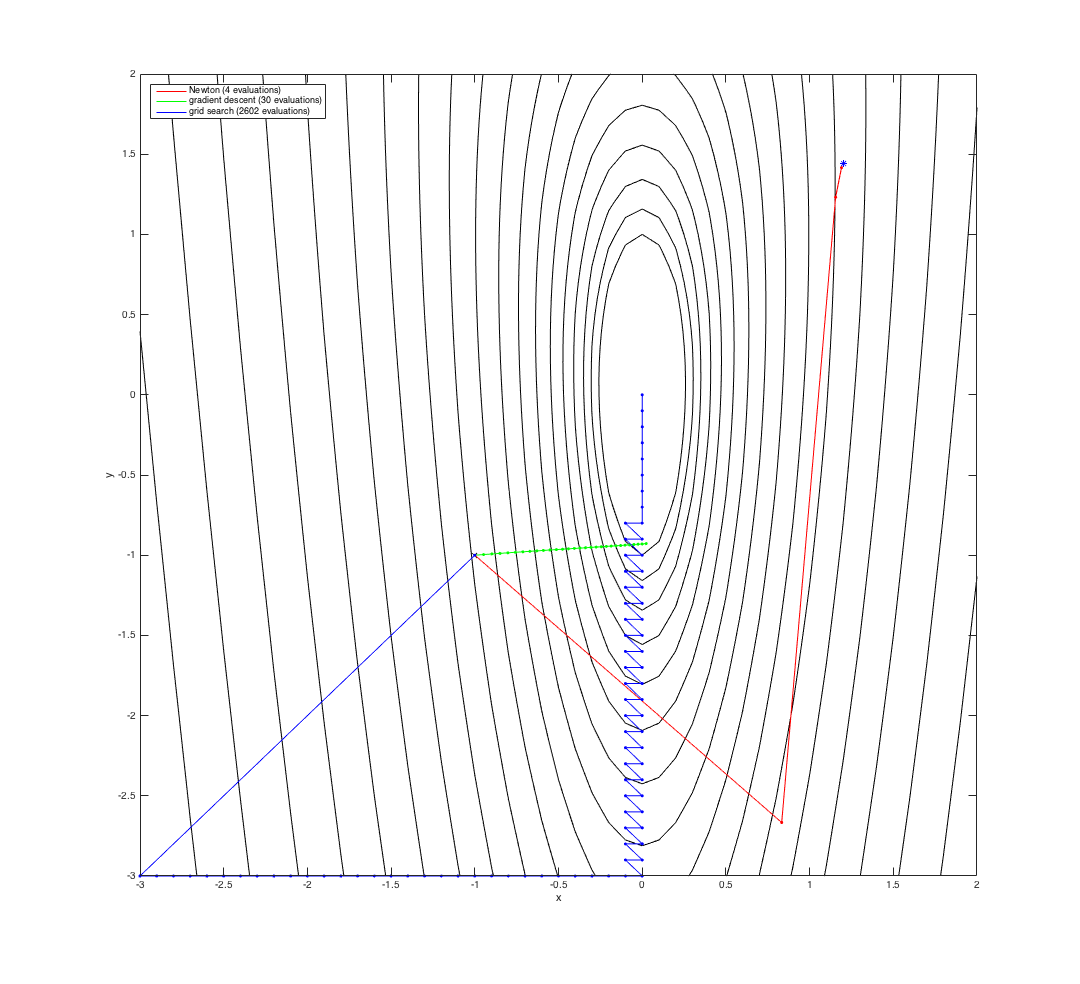
\includegraphics[scale=0.5]{code/2c.png}

\section*{Problem 2(d)}

The grid search method failed to converge in the maximum number of iterations allowed; it converged in 2602 iterations.

\section*{Problem 2(e)}

Newton's method took the fewest iterations (4 iterations).

\section*{Problem 2(f)}

TODO

\section*{Problem 2(g)}

TODO

\section*{Problem 2(h)}

TODO

\end{document}